\chapter{Calcul algébrique}

\section{Somme et produit}

\begin{defin}
	Une \textbf{somme} est le résultat d'une addition. Les éléments que l'on additionne s'appellent des \textbf{termes}.

	Une \textbf{différence} est le résultat d'une soustraction. Tout comme la somme, elle est composée de \textbf{termes}.

	Un \textbf{produit} est le résultat d'une multiplication. Les éléments que l'on multiplie s'appellent des \textbf{facteurs}.

	Un \textbf{quotient} est le résultat d'une division. Il est composé d'un \textbf{numérateur} et d'un \textbf{dénominateur}.
\end{defin}

\begin{attention}
	Contrairement aux autres opérations, un quotient n'existe que si son dénominateur est \textbf{différent de zéro}.
	\[
		\frac{A}{B} \text{ n'existe que si } B \neq 0
	\]
\end{attention}

\begin{rem}
	Le produit et le quotient suivent la même règle :
	\begin{itemize}
		\item Signes identiques $\Rarr$ résultat positif ($+$).
		\item Signes contraires $\Rarr$ résultat négatif ($-$).
	\end{itemize}
\end{rem}

\begin{ex}
	\nline
	\begin{multicols}{3}
		\textbf{Sommes (ou différences)}
		\begin{itemize}
			\item $x - 3$
			\item $(2x + 4) + 3x$
			\item $(5 - x) - (9 + 9x)$
			\item $3 + (2 + 3x)(x - 2)$
		\end{itemize}

		\columnbreak

		\textbf{Produits de facteurs}
		\begin{itemize}
			\item $(6x + 1) \times (x - 1)$
			\item $2 \times (1 + 6x)$
			\item $(8 - x) \times (2 + x)$
			\item $(3 + 8x) \times (x - 8)^2$
		\end{itemize}

		\columnbreak

		\textbf{Quotients (num./dén.)}
		\begin{itemize}
			\item $\dfrac{x+3}{2}$
			\item $\dfrac{5}{x-1}$
			\item $\dfrac{3x^2+1}{2x-4}$
			      % \item $\dfrac{(x+1)(x-3)}{x^2+5}$
		\end{itemize}
	\end{multicols}
\end{ex}

\begin{defin}[Développer et factoriser]
	\nline
	\begin{itemize}
		\item \textbf{Développer} c'est transformer un produit (ou quotient) en une somme (ou différence).
		\item \textbf{Factoriser} c'est transformer une somme (ou différence) en un produit (ou quotient).
	\end{itemize}
	\ms
	\begin{center}
		\begin{tikzpicture}[
			transform shape,
			block/.style={ rectangle, rounded corners=4pt, very thick, text centered, minimum width=11em, minimum height=3em, text width=10.5em, inner sep=3pt, font=\bfseries\large },
			block_sum/.style={ block, draw=red!75, fill=red!5 },
			block_prod/.style={block, draw=green!60!black, fill=green!5},
			arrow/.style={-{Stealth[scale=1.0]}, thick, shorten >=2pt, shorten <=2pt}
			]
			\node (product) [block_prod] {PRODUIT \\ (ou Quotient)};
			\node (sum) [block_sum, right=2.5cm of product] {SOMME \\ (ou Différence)};
			\draw [arrow, out=30, in=150] (product.north) to (sum.north);
			\path [decorate, decoration={text along path, text={D{é}velopper}, text align=center, raise=5pt}] (product.north) [out=30, in=150] to (sum.north);
			\draw [arrow, out=210, in=330] (sum.south) to (product.south);
			\path [decorate, decoration={text along path, text={Factoriser}, text align=center, raise=-15pt}] (product.south) [out=330, in=210] to (sum.south);
		\end{tikzpicture}
	\end{center}
\end{defin}

\newpage

\section{Développement}

\begin{prop}[Distributivité]
	Soient $a$, $b$ et $c$ trois nombres réels. On a :
	\begin{center}
		\begin{tikzpicture}[transform shape,arrow/.style={-{Stealth[scale=0.8]}, thick, color=blue!70!black},node distance=0.1cm ]
			\node (expr) {\Large $a(b + c) = ab + ac$};
			\path (expr.west) ++(0.35, 0.2) node (a_pos) {};
			\path (expr.west) ++(0.85, 0.2) node (b_pos) {};
			\path (expr.west) ++(1.7, 0.2) node (c_pos) {};
			\draw [arrow] (a_pos.center) to[out=85, in=95, distance=4mm] (b_pos.center);
			\draw [arrow] (a_pos.center) to[out=85, in=95, distance=7mm] (c_pos.center);
		\end{tikzpicture}
	\end{center}
\end{prop}

\begin{methode}[Développer une expression]
	Développer les expressions suivantes :
	\begin{multicols}{3}
		\begin{itemize}
			\item $A = 4(5 + x)$
			\item $B = 5(x - 2)$
			\item $C = (4x + 6) \times 3$
			\item $D = -6(-2x + 4)$
			\item $E = -x(2 - 3x)$
			\item $F = -(5 - x)$
		\end{itemize}
	\end{multicols}

	\begin{correction}
		\[
			\begin{array}{lll}%
				\def\arraystretch{1.3}%
				\begin{array}{rcl}%
					A & = & 4(5 + x) \\
					  & = & 20 + 4x  \\
				\end{array} \quad  & \quad  %
				\def\arraystretch{1.3}%
				\begin{array}{rcl}%
					B & = & 5(x - 2) \\
					  & = & 5x - 10  \\
				\end{array} \quad  & \quad  %
				\def\arraystretch{1.3}%
				\begin{array}{rcl}%
					C & = & (4x + 6) \times 3 \\
					  & = & 12x + 18          \\
				\end{array} \\&&\\%
				\def\arraystretch{1.3}%
				\begin{array}{rcl}%
					D & = & -6(-2x + 4) \\
					  & = & 12x - 24    \\
				\end{array} \quad & \quad %
				\def\arraystretch{1.3}%
				\begin{array}{rcl}%
					E & = & -x(2 - 3x) \\
					  & = & -2x + 3x^2 \\
				\end{array} \quad & \quad %
				\def\arraystretch{1.3}%
				\begin{array}{rcl}%
					F & = & -(5 - x) = -1(5 - x) \\
					  & = & -5 + x               \\
				\end{array}%
			\end{array}%
		\]
		\textit{Un signe $\pa{-}$ devant une parenthèse change les signes dans la parenthèse.}
	\end{correction}
\end{methode}

\begin{prop}[Double distributivité]
	Soient $a$, $b$, $c$ et $d$ quatre nombres réels. On a :
	\begin{center}
		\begin{tikzpicture}[transform shape,arrow_a/.style={-{Stealth[scale=0.8]}, thick, color=blue!70!black},arrow_b/.style={-{Stealth[scale=0.8]}, thick, color=red!70!black},node distance=0.1cm ]
			\node (expr) {\Large $(a + b)(c + d) = ac + ad + bc + bd$};
			\path (expr.west) ++(0.45, 0.2) node (a_top) {};
			\path (expr.west) ++(2.05, 0.2) node (c_top) {};
			\path (expr.west) ++(2.85, 0.2) node (d_top) {};
			\path (expr.west) ++(1.45, -0.2) node (b_bot) {};
			\path (expr.west) ++(2.05, -0.2) node (c_bot) {};
			\path (expr.west) ++(2.85, -0.2) node (d_bot) {};
			\draw [arrow_a] (a_top.center) to[out=80, in=100, distance=6mm] (c_top.center);
			\draw [arrow_a] (a_top.center) to[out=85, in=95, distance=11mm] (d_top.center);
			\draw [arrow_b] (b_bot.center) to[out=-80, in=-100, distance=5mm] (c_bot.center);
			\draw [arrow_b] (b_bot.center) to[out=-85, in=-95, distance=9mm] (d_bot.center);
		\end{tikzpicture}
	\end{center}
\end{prop}

\begin{methode}[Développer et réduire par double distributivité]
	Développer et réduire :
	\begin{multicols}{2}
		\begin{itemize}
			\item $A = (2x + 3)(x + 8)$
			\item $B = (-3 + x)(4 - 5x)$
			\item $C = 2(3 + x)(3 - 2x)$
			\item $D = 2x(1 - x) - (x - 3)(3x + 2)$
		\end{itemize}
	\end{multicols}

	\begin{correction}
		\[
			\begin{array}{ll}%
				\def\arraystretch{1.3}%
				\begin{array}{rcl}%
					A & = & (2x + 3)(x + 8)      \\
					  & = & 2x^2 + 16x + 3x + 24 \\
					  & = & 2x^2 + 19x + 24      \\
				\end{array}  \quad & \quad %
				\def\arraystretch{1.3}%
				\begin{array}{rcl}%
					B & = & (-3 + x)(4 - 5x)      \\
					  & = & -12 + 15x + 4x - 5x^2 \\
					  & = & -5x^2 + 19x - 12      \\
				\end{array} \\ & \\%
				\def\arraystretch{1.3}%
				\begin{array}{rcl}%
					C & = & 2(3 + x)(3 - 2x)      \\
					  & = & 2(9 - 6x + 3x - 2x^2) \\
					  & = & 2(-2x^2 - 3x + 9)     \\
					  & = & -4x^2 - 6x + 18       \\
				\end{array}  \quad & \quad %
				\def\arraystretch{1.3}%
				\begin{array}{rcl}%
					D & = & 2x(1 - x) - (x - 3)(3x + 2)      \\
					  & = & 2x - 2x^2 - (3x^2 + 2x - 9x - 6) \\
					  & = & 2x - 2x^2 - 3x^2 - 2x + 9x + 6   \\
					  & = & -5x^2 + 9x + 6                   \\
				\end{array}%
			\end{array}%
		\]
	\end{correction}
\end{methode}
\newpage

\section{Factorisation}

\begin{methode}[Factoriser par facteur commun (1)]
	Trouver le facteur commun, puis factoriser et réduire si possible :
	\begin{multicols}{3}
		\begin{itemize}
			\item $A = 3{,}5x - 4{,}2x + 2{,}1x$
			\item $B = 4t - 5tx + 3t$
			\item $C = 4x - 4y + 8$
			\item $D = x^2 + 3x - 5x^2$
			\item $E = 3t + 9u + 3$
			\item $F = 3x^2 - x$
		\end{itemize}
	\end{multicols}

	\begin{correction}
		\[
			\begin{array}{lll}%
				\def\arraystretch{1.3}%
				\begin{array}{rcl}%
					A & = & x(3{,}5 - 4{,}2 + 2{,}1) \\
					  & = & 1{,}4x
				\end{array}\quad & \quad %
				\def\arraystretch{1.3}%
				\begin{array}{rcl}%
					B & = & t(4 - 5x + 3) \\
					  & = & t(7 - 5x)
				\end{array}\quad & \quad %
				\def\arraystretch{1.3}%
				\begin{array}{rcl}%
					C & = & 4x - 4y + 4 \times 2 \\
					  & = & 4(x - y + 2)
				\end{array} \\~&~&~\\%
				\def\arraystretch{1.3}%
				\begin{array}{rcl}%
					D & = & x(x + 3 - 5x) \\
					  & = & x(-4x + 3)
				\end{array}\quad & \quad %
				\def\arraystretch{1.3}%
				\begin{array}{rcl}%
					E & = & 3(t + 3u + 1) \\
					  &   &               \\
				\end{array}\quad & \quad %
				\def\arraystretch{1.3}%
				\begin{array}{rcl}%
					F & = & x(3x - 1) \\
					  &   &           \\
				\end{array}%
			\end{array}%
		\]
	\end{correction}
\end{methode}

\begin{methode}[Factoriser par facteur commun (2)]
	Factoriser les expressions suivantes :
	\begin{multicols}{3}
		\begin{itemize}
			\item $A = 3(2 + 3x) - (5 + 2x)(2 + 3x)$
			\item $B = (2 - 5x)^2 - (2 - 5x)(1 + x)$
			\item $C = 5(1 - 2x) - (4 + 3x)(2x - 1)$
		\end{itemize}
	\end{multicols}

	\begin{correction}
		\[
			\begin{array}{ll}%
				\def\arraystretch{1.3}%
				\begin{array}{rcl}%
					A & =                                                 & 3(2 + 3x) - (5 + 2x)(2 + 3x) \\
					  & \multicolumn{2}{l}{\text{Facteur commun : } 2+3x}                                \\
					  & =                                                 & (2 + 3x)(3 - (5 + 2x))       \\
					  & =                                                 & (2 + 3x)(3 - 5 - 2x)         \\
					  & =                                                 & (2 + 3x)(-2 - 2x)            \\
					  &                                                   &                              \\
				\end{array} \quad & \quad %
				\def\arraystretch{1.3}%
				\begin{array}{rcl}%
					B & =                                                 & (2 - 5x)^2 - (2 - 5x)(1 + x)       \\
					  & =                                                 & (2 - 5x)(2 - 5x) - (2 - 5x)(1 + x) \\
					  & \multicolumn{2}{l}{\text{Facteur commun : } 2-5x}                                      \\
					  & =                                                 & (2 - 5x)((2 - 5x) - (1 + x))       \\
					  & =                                                 & (2 - 5x)(2 - 5x - 1 - x)           \\
					  & =                                                 & (2 - 5x)(1 - 6x)                   \\
				\end{array}%
			\end{array}%
		\]
		\ms
		On modifie l'écriture de $C$ pour faire apparaître un facteur commun : $(2x - 1) = -(1 - 2x)$
		\[
			\def\arraystretch{1.3}%
			\begin{array}{rcl}%
				C & =                                                 & 5(1 - 2x) - (4 + 3x)(2x - 1) \\
				  & =                                                 & 5(1 - 2x) + (4 + 3x)(1 - 2x) \\
				  & \multicolumn{2}{l}{\text{Facteur commun : } 1-2x}                                \\
				  & =                                                 & (1 - 2x)(5 + (4 + 3x))       \\
				  & =                                                 & (1 - 2x)(9 + 3x)             \\
			\end{array}%
		\]
	\end{correction}
\end{methode}

\newpage

\section{Identités remarquables}

\begin{prop}[Les trois identités remarquables]
	\[
		\boxed{(a+b)^2 = a^2 + 2ab + b^2} \qquad\qquad \boxed{(a-b)^2 = a^2 - 2ab + b^2} \qquad\qquad \boxed{(a+b)(a-b) = a^2 - b^2}
	\]
\end{prop}

\begin{ex}
	\[
		\begin{array}{ll}%
			\begin{array}{rcccccl}%
				(x + 3)^2 & = & x^2 & + & 2 \times x \times 3 & + & 3^2 \\
				          & = & x^2 & + & 6x                  & + & 9   \\
			\end{array}\qquad & \qquad %
			\begin{array}{rcccccl}%
				(x - 5)^2 & = & x^2 & - & 2 \times x \times 5 & + & 5^2 \\
				          & = & x^2 & - & 10x                 & + & 25  \\
			\end{array} \\ & \\%
			\begin{array}{rcccl}%
				(2x - 1)(2x + 1) & = & (2x)^2 & - & 1^2 \\
				                 & = & 4x^2   & - & 1
			\end{array}\qquad      & \qquad~    %
		\end{array}%
	\]
\end{ex}

\subsection{Développer avec les identités remarquables}

\begin{methode}[Développer avec les identités remarquables (1)]
	Développer et réduire éventuellement :
	\begin{multicols}{3}
		\begin{itemize}
			\item $A = (x + 3)^2$
			\item $B = (3x - 4)^2$
			\item $C = (x - 3)(x + 3)$
			\item $D = (2x + 3)(2x - 3)$
			\item $E = (4 - 3x)(3x + 4)$
		\end{itemize}
	\end{multicols}

	\begin{correction}
		\[
			\begin{array}{lll}%
				\def\arraystretch{1.3}%
				\begin{array}{rcl}%
					A & = & (x + 3)^2    \\
					  & = & x^2 + 6x + 9 \\
				\end{array} \quad & \quad %
				\def\arraystretch{1.3}%
				\begin{array}{rcl}%
					B & = & (3x - 4)^2      \\
					  & = & 9x^2 - 24x + 16 \\
				\end{array} \quad & \quad %
				\def\arraystretch{1.3}%
				\begin{array}{rcl}%
					C & = & (x - 3)(x + 3) \\
					  & = & x^2 - 9        \\
				\end{array} \\&\\%
				\def\arraystretch{1.3}%
				\begin{array}{rcl}%
					D & = & (2x + 3)(2x - 3) \\
					  & = & 4x^2 - 9         \\
					  &   &                  \\
				\end{array} \quad & \quad %
				\def\arraystretch{1.3}%
				\begin{array}{rcl}%
					E & = & (4 - 3x)(3x + 4) \\
					  & = & (4 - 3x)(4 + 3x) \\
					  & = & 16 - 9x^2        \\
				\end{array} & ~ %
			\end{array}%
		\]
	\end{correction}
\end{methode}

\begin{methode}[Développer avec les identités remarquables (2)]
	Développer et réduire :
	\begin{multicols}{3}
		\begin{itemize}
			\item $A = (2x - 3)^2 + (x + 5)(3 - x)$
			\item $B = (x - 3)(x + 3) - (4 - 3x)^2$
			\item $C = 2(x + 3) + (2x + 3)(2x - 3)$
		\end{itemize}
	\end{multicols}

	\begin{correction}
		\[
			\begin{array}{ll}%
				\def\arraystretch{1.3}%
				\begin{array}{rcl}%
					A & = & (2x - 3)^2 + (x + 5)(3 - x)         \\
					  & = & 4x^2 - 12x + 9 + 3x - x^2 + 15 - 5x \\
					  & = & 3x^2 - 14x + 24                     \\
					  &   &                                     \\
				\end{array} \quad & \quad %
				\def\arraystretch{1.3}%
				\begin{array}{rcl}%
					B & = & (x - 3)(x + 3) - (4 - 3x)^2 \\
					  & = & x^2 - 9 - (16 - 24x + 9x^2) \\
					  & = & x^2 - 9 - 16 + 24x - 9x^2   \\
					  & = & -8x^2 + 24x - 25            \\
				\end{array} \\%
				\def\arraystretch{1.3}%
				\begin{array}{rcl}%
					C & = & 2(x + 3) + (2x + 3)(2x - 3) \\
					  & = & 2x + 6 + 4x^2 - 9           \\
					  & = & 4x^2 + 2x - 3               \\
				\end{array}        \quad & \quad ~ %
			\end{array}%
		\]
	\end{correction}
\end{methode}

\newpage

\subsection{Factoriser avec les identités remarquables}

\begin{methode}[Factoriser avec les identités remarquables (1)]
	Factoriser :
	\begin{multicols}{3}
		\begin{itemize}
			\item $A = x^2 - 2x + 1$
			\item $B = 4x^2 + 12x + 9$
			\item $C = 9x^2 - 4$
			      % \item $D = 25 + 16x^2 - 40x$
			      % \item $E = 1 - 49x^2$
		\end{itemize}
	\end{multicols}

	\begin{correction}
		On identifie les termes $a^2$, $2ab$, $b^2$ des identités remarquables.
		\[
			\begin{array}{lll}%
				\def\arraystretch{1.3}%
				\begin{array}{rcl}%
					A & =                                                                            & x^2 - 2x + 1 \\
					  & \multicolumn{2}{l}{\quad\Rarr a=x,\ b=1 \quad\text{ (2}^\text{e}\text{ IR)}}                \\
					  & =                                                                            & (x - 1)^2    \\
					  &                                                                              &              \\
				\end{array}                         &                         %
				\def\arraystretch{1.3}%
				\begin{array}{rcl}%
					B & =                                                                              & 4x^2 + 12x + 9                      \\
					  & =                                                                              & (2x)^2 + 2 \times 2x \times 3 + 3^2 \\
					  & \multicolumn{2}{l}{\quad\Rarr a=2x,\ b=3 \quad\text{ (1}^\text{re}\text{ IR)}}                                       \\
					  & =                                                                              & (2x + 3)^2                          \\
				\end{array} & %
				\def\arraystretch{1.3}%
				\begin{array}{rcl}%
					C & =                                                                             & 9x^2 - 4         \\
					  & =                                                                             & (3x)^2 - 2^2     \\
					  & \multicolumn{2}{l}{\quad\Rarr a=3x,\ b=2 \quad\text{ (3}^\text{e}\text{ IR)}}                    \\
					  & =                                                                             & (3x - 2)(3x + 2) \\
				\end{array}%
			\end{array}%
		\]
	\end{correction}
\end{methode}

\begin{methode}[Factoriser avec les identités remarquables (2)]
	Factoriser et réduire :
	\begin{multicols}{3}
		\begin{itemize}
			\item $A = (2x + 3)^2 - 64$
			\item $B = 1 - (2 - 5x)^2$
		\end{itemize}
	\end{multicols}

	\begin{correction}
		\[
			\begin{array}{ll}%
				\def\arraystretch{1.3}%
				\begin{array}{rcl}%
					A & =                                                                               & (2x + 3)^2 - 64              \\
					  & =                                                                               & (2x + 3)^2 - 8^2             \\
					  & \multicolumn{2}{l}{\quad\Rarr a=2x+3,\ b=8 \quad\text{ (3}^\text{e}\text{ IR)}}                                \\
					  & =                                                                               & ((2x + 3) - 8)((2x + 3) + 8) \\
					  & =                                                                               & (2x - 5)(2x + 11)            \\
					  &                                                                                 &                              \\
				\end{array} \quad & \quad %
				\def\arraystretch{1.3}%
				\begin{array}{rcl}%
					B & =                                                                               & 1 - (2 - 5x)^2               \\
					  & =                                                                               & 1^2 - (2 - 5x)^2             \\
					  & \multicolumn{2}{l}{\quad\Rarr a=1,\ b=2-5x \quad\text{ (3}^\text{e}\text{ IR)}}                                \\
					  & =                                                                               & (1 - (2 - 5x))(1 + (2 - 5x)) \\
					  & =                                                                               & (1 - 2 + 5x)(1 + 2 - 5x)     \\
					  & =                                                                               & (-1 + 5x)(3 - 5x)            \\
				\end{array}%
			\end{array}%
		\]
	\end{correction}
\end{methode}

\begin{rem}[Identité remarquable sous forme graphique]
	\nline
	\begin{center}
		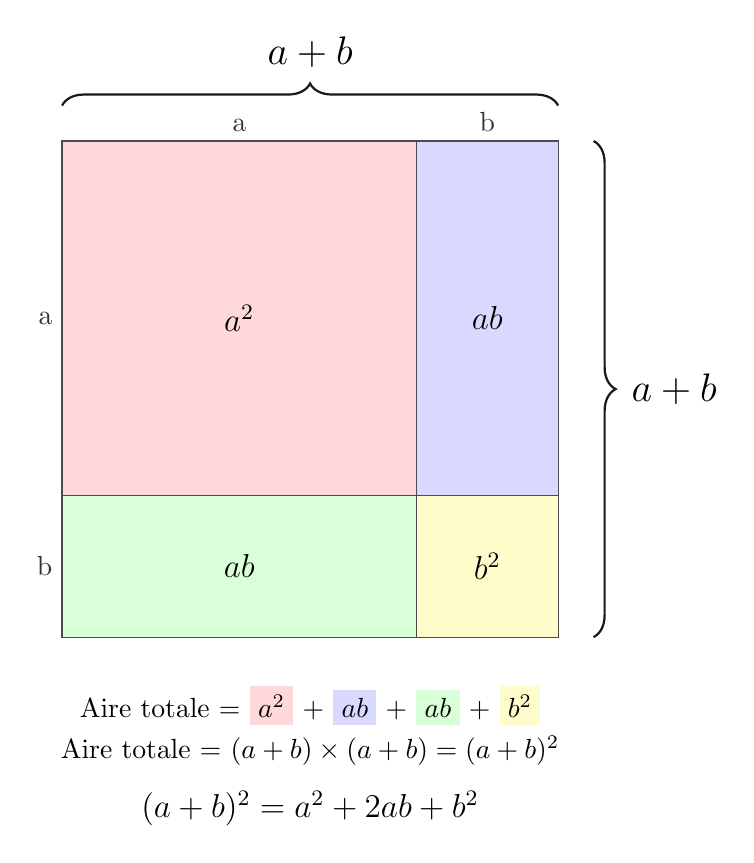
\begin{tikzpicture}[scale=1.5,font=\bfseries\large,quad/.style={draw=black!70,thin},label_side/.style={font=\normalfont\normalsize,color=black!80}]
			\def\la{3.0} \def\lb{1.2} \draw[quad, fill=red!15] (0,\lb) rectangle (\la, {\la+\lb}) node[pos=0.5] {$a^2$};
			\draw[quad, fill=blue!15] (\la,\lb) rectangle ({\la+\lb}, {\la+\lb}) node[pos=0.5] {$ab$};
			\draw[quad, fill=green!15] (0,0) rectangle (\la,\lb) node[pos=0.5] {$ab$};
			\draw[quad, fill=yellow!20] (\la,0) rectangle ({\la+\lb},\lb) node[pos=0.5] {$b^2$};
			\node[label_side, above] at ({\la/2}, {\la+\lb}) {a};
			\node[label_side, above] at ({\la+\lb/2}, {\la+\lb}) {b};
			\node[label_side, left] at (0, {\lb+\la/2}) {a};
			\node[label_side, left] at (0, {\lb/2}) {b};
			\draw[decorate, decoration={brace, amplitude=8pt}, thick, draw=black!90] (0, {\la+\lb+0.3}) -- ({\la+\lb}, {\la+\lb+0.3}) node[midway, above=10pt, font=\bfseries\Large, color=black] {$a + b$};
			\draw[decorate, decoration={brace, amplitude=8pt, mirror}, thick, draw=black!90] ({\la+\lb+0.3}, 0) -- ({\la+\lb+0.3}, {\la+\lb}) node[midway, right=10pt, font=\bfseries\Large, color=black] {$a + b$};
			\node[anchor=north, align=center, font=\normalfont\normalsize, yshift=-0.5cm] at ({(\la+\lb)/2}, 0) { Aire totale = \colorbox{red!15}{$a^2$} + \colorbox{blue!15}{$ab$} + \colorbox{green!15}{$ab$} + \colorbox{yellow!20}{$b^2$} \\[1mm] Aire totale = $(a + b) \times (a + b) = (a + b)^2$\\[3mm] \large $\Rarr (a + b)^2 = a^2 + 2ab + b^2$ };
		\end{tikzpicture}
	\end{center}
\end{rem}
